%%
%% This is file `sample-sigconf.tex',
%% generated with the docstrip utility.
%%
%% The original source files were:
%%
%% samples.dtx  (with options: `sigconf')
%%
%% IMPORTANT NOTICE:
%%
%% For the copyright see the source file.
%%
%% Any modified versions of this file must be renamed
%% with new filenames distinct from sample-sigconf.tex.
%%
%% For distribution of the original source see the terms
%% for copying and modification in the file samples.dtx.
%%
%% This generated file may be distributed as long as the
%% original source files, as listed above, are part of the
%% same distribution. (The sources need not necessarily be
%% in the same archive or directory.)
%%
\PassOptionsToPackage{dvipsnames}{xcolor}
%% The first command in your LaTeX source must be the \documentclass command.
\documentclass[sigconf]{acmart}
\settopmatter{printacmref=false} % Removes citation information below abstract
\renewcommand\footnotetextcopyrightpermission[1]{} % removes footnote with conference information in first column
\pagestyle{plain} % removes running headers

\usepackage{amsmath,amssymb,amsfonts}
\usepackage{graphicx}
\usepackage{textcomp}
%\usepackage[dvipsnames]{xcolor}
\usepackage{minted}
\usepackage{caption}
\usepackage{subcaption}
\usepackage{booktabs}
\usepackage{tikz-timing}
\usepackage{microtype}
\usepackage{float}
\usetikztiminglibrary{arrows}
\usetikztiminglibrary[rising arrows]{clockarrows}
\usetikztiminglibrary{nicetabs}

\usepackage{algorithm}
\usepackage[noend]{algpseudocode}

\graphicspath{{./figs/}}

%%
%% \BibTeX command to typeset BibTeX logo in the docs
\AtBeginDocument{%
  \providecommand\BibTeX{{%
    \normalfont B\kern-0.5em{\scshape i\kern-0.25em b}\kern-0.8em\TeX}}}

%% Rights management information.  This information is sent to you
%% when you complete the rights form.  These commands have SAMPLE
%% values in them; it is your responsibility as an author to replace
%% the commands and values with those provided to you when you
%% complete the rights form.
\acmConference[290 Project]{}{}{}

%%
%% Submission ID.
%% Use this when submitting an article to a sponsored event. You'll
%% receive a unique submission ID from the organizers
%% of the event, and this ID should be used as the parameter to this command.
%%\acmSubmissionID{123-A56-BU3}

%%
%% The majority of ACM publications use numbered citations and
%% references.  The command \citestyle{authoryear} switches to the
%% "author year" style.
%%
%% If you are preparing content for an event
%% sponsored by ACM SIGGRAPH, you must use the "author year" style of
%% citations and references.
%% Uncommenting
%% the next command will enable that style.
%%\citestyle{acmauthoryear}

%%
%% end of the preamble, start of the body of the document source.
\begin{document}

%%
%% The "title" command has an optional parameter,
%% allowing the author to define a "short title" to be used in page headers.
%\title{The Name of the Title is Hope}
\title{Power Modeling and Estimation for Gemmini}

%%
%% The "author" command and its associated commands are used to define
%% the authors and their affiliations.
%% Of note is the shared affiliation of the first two authors, and the
%% "authornote" and "authornotemark" commands
%% used to denote shared contribution to the research.
\author{Vighnesh Iyer}
\email{vighnesh.iyer@berkeley.edu}
\affiliation{%
  \institution{University of California, Berkeley}
}

\author{Billy Chau}
\email{chunheichau@berkeley.edu}
\affiliation{%
  \institution{University of California, Berkeley}
}

%%
%% By default, the full list of authors will be used in the page
%% headers. Often, this list is too long, and will overlap
%% other information printed in the page headers. This command allows
%% the author to define a more concise list
%% of authors' names for this purpose.
%\renewcommand{\shortauthors}{Trovato and Tobin, et al.}

%%
%% The abstract is a short summary of the work to be presented in the
%% article.
\begin{abstract}
  This project seeks to develop an architectural power model for Gemmini based on a macroblock characterization flow.
  The power model will be validated against synthesized implementations of Gemmini running microbenchmarks.
  The model will be used to evaluate the energy breakdown of more complex software and benchmark Gemmini against other ML accelerators.
\end{abstract}

\maketitle

\section{Background and Prior Work}
There are several techniques used in prior work to evaluate power metrics for a digital architecture.
These techniques can be compared and contrasted across the visibility/granularity, fidelity/accuracy, speed, and startup time axes as shown in table \ref{}.

\subsection{Architecture-level Power Modeling}\label{arch_modeling}
This technique typically involves embedding a power model into a functional model of a digital design, or by simulating an abstract architecture description against an abstract software model/activity counts.

Examples for the former technique include the power models used for evaluating the Eyeriss v2\cite{eyerissv2} and SCNN\cite{scnn} architectures which were implemented by counting SRAM reads/writes, MACs, NoC metrics, and DRAM accesses within the functional model, and assigning an energy/op number to each type of op.
Some refinements to the power model were made by accounting for the impact of sparsity on MAC power (clock gating), the power usage of crossbars, FIFOs, and other auxiliary control circuits, and using a cycle-accurate performance model to capture non-idealities such as DRAM and NoC latency and multi-cycle arithmetic.

An example of the latter technique is Accelergy\cite{accelergy}, which is a framework for estimating power from an architectural description of a tiled PE accelerator, a description of the digital components for that architecture (SRAMs, registers, MAC/multiply/adder blocks, FIFOs, crossbars, NoC routers, etc.), and plugins for defining the power models of each architectural component depending on what actions are performed on them.
Accelergy is fed by a performance model which produces activity counts accounting for memory, compute, and communication latencies.
Another example of an architectural power model using an abstract architecture description is the gem5 power simulator\cite{gem5power}.

Architecture-level modeling is generally fast, but can suffer from low accuracy if $\mu$Arch details aren't properly considered or if the per-component power models aren't properly characterized. However, for ML accelerators, due to the regularity of computation and memory movement, architecture power models can be quite accurate. In the context of Gemmini, such a model may have accuracy loss due to non-consideration of CPU power, and performance variation from SoC integration (the effect of the shared L2 cache with the CPU, the impact of coherence from L1 and fencing, threading, and interrupts).

\subsubsection{RTL Macromodeling}
To generate the component-level power models for use in architectural simulation, RTL macromodeling is used.
The idea is to create a function ($f(\text{input statistic}) = \text{predicted energy}$) that can map some statistics about the input to a macroblock to the energy consumed by the block to process the input.
Concretely, this would be a map from input data sparsity to dynamic energy for an arithmetic block, a fixed cost model for SRAMs (accounting for re-reading the same address), and an activity-based model for registers.
The model also accounts for leakage energy that is expended every cycle.

\subsection{Post-Synthesis Vectored Power Simulation}\label{syn_modeling}
This flow is supported by Cadence Joules and involves taking an RTL design through synthesis and measuring power from a VCD generated by gate-level simulation.
This technique is relatively fast compared to the signoff power flow, but requires a full RTL design and a synthesized netlist.
It is relatively accurate, but can only estimate the layout parasitics from a partial sketch of the floorplan.

\subsection{Post-PnR Vectored Power Simulation}
This flow is supported by Cadence Voltus and requires the RTL to be fully implemented to function; furthermore a post-pnr gate-level sim is required which runs very slowly (~100 Hz).
However, the signoff power estimated by this flow is as accurate as one can get and you can get precise current waveforms for each net.

\subsection{Chip measurement}
Taking an architecture to tapeout will get the most accurate power numbers, will be able to run software in realtime, but you will only be able to evaluate a few corners, supplies, and frequencies with only one design point.
A chip also has poor visibility and getting module-level power numbers is not possible.

\section{Approach and Results}

\subsection{Proposed Flow}
We propose a flow that combines the techniques from Sections \ref{arch_modeling} and \ref{syn_modeling} in Figure \ref{fig:overall_flow}.
We set out to perform macroblock power characterization on the most power hungry units of Gemmini (MAC, registers, and SRAM), apply those numbers to an embedded power model in Gemmini's functional simulator, validate the power estimates from the arch power simulator against post-synthesis power estimation, and finally attempt to model Gemmini in Accelergy as an additional point of validation.

\begin{figure}
  \begin{center}
    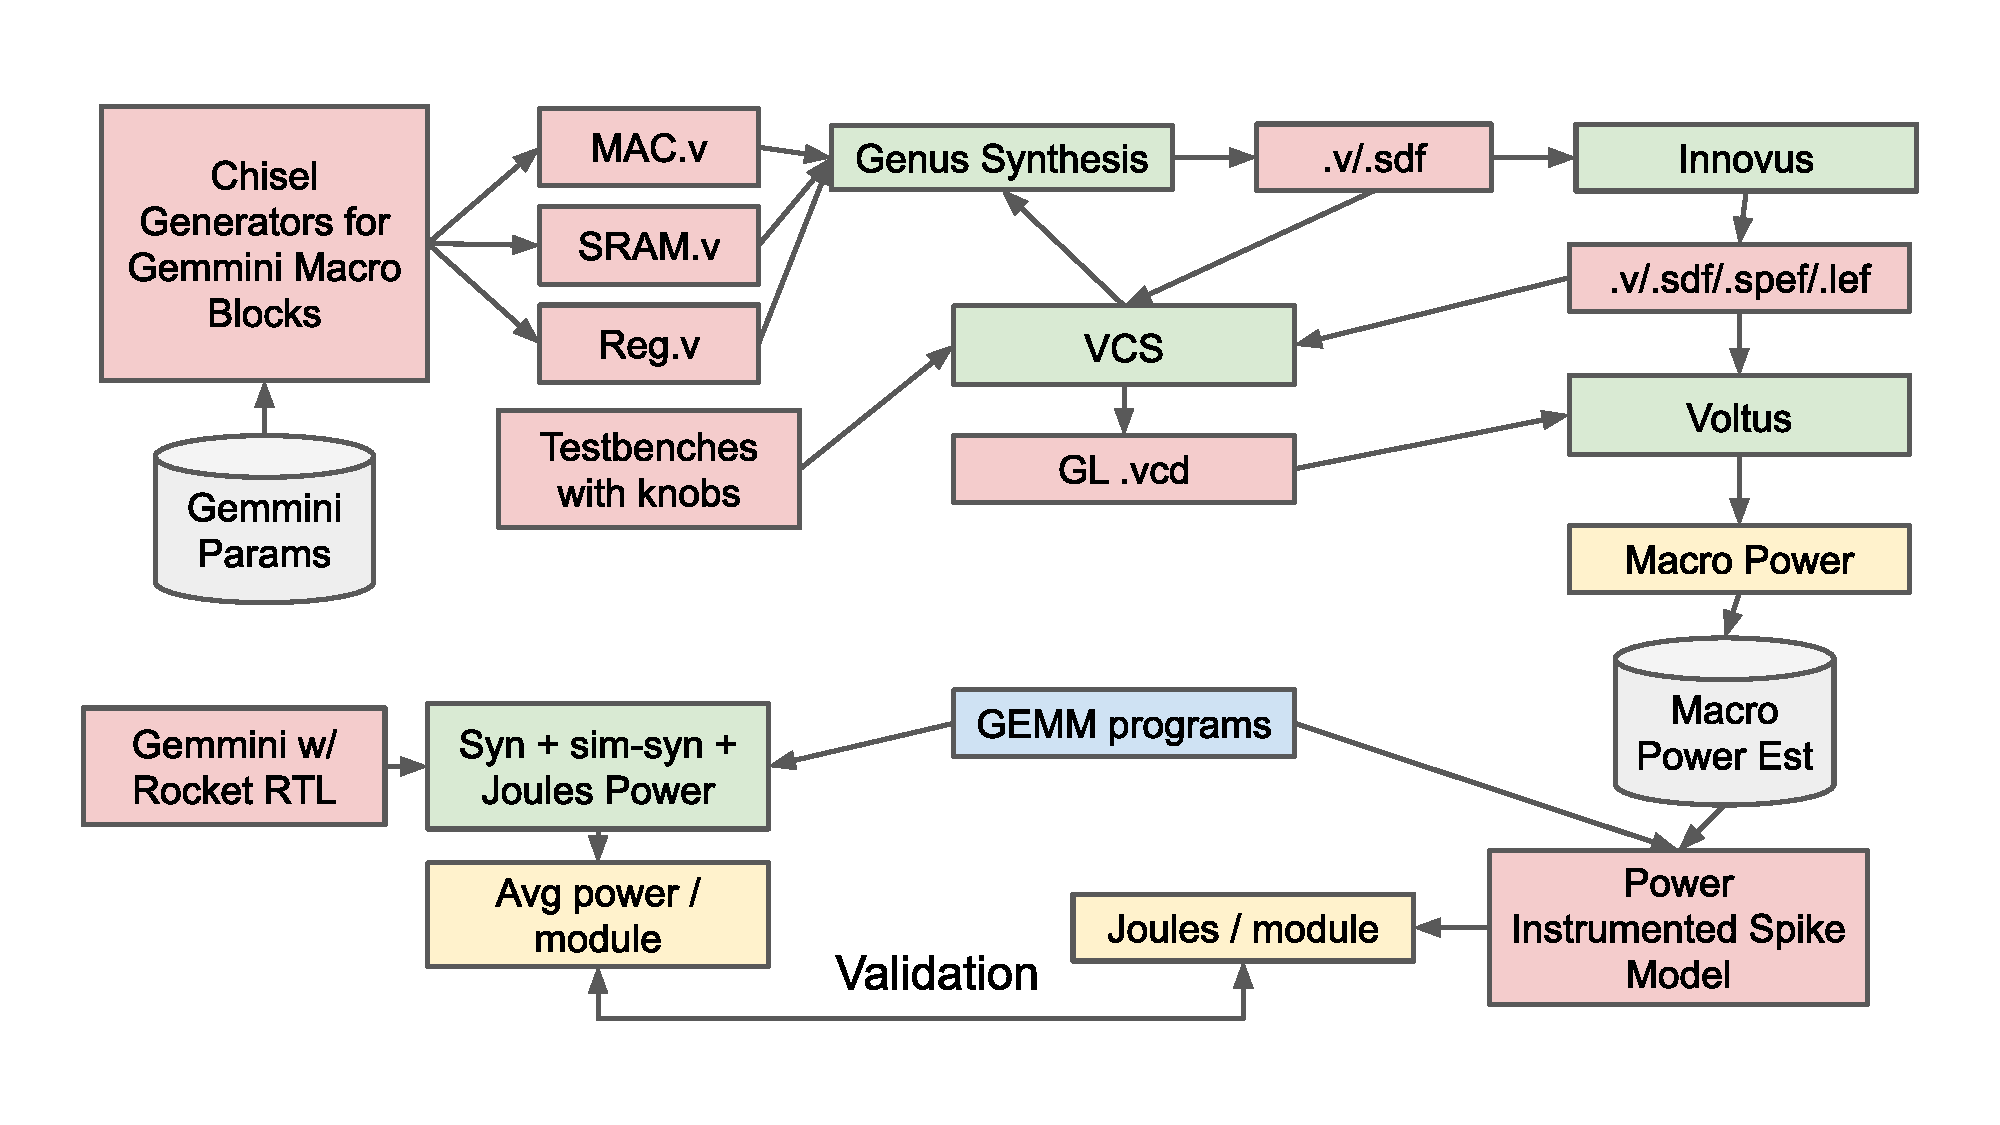
\includegraphics[width=\linewidth]{overall_flow.pdf}
  \end{center}
  \caption{Description of the proposed flow consisting of macroblock modeling, activity instrumentation of a functional model, and validation with Joules}
\end{figure}

\subsection{Macroblock Power Modeling}
We propose macroblock modeling of a few power-critical blocks of Gemmini such as the MAC and SRAM units that make up the accumulator and scratchpad.
We can extract the register write energy from the MAC macromodeling as described below.

The macroblock modeling flow starts with Chisel generators that mimic the power-critical modules of Gemmini and are parameterized similar to Gemmini.
These blocks are pushed through the standard VLSI flow to produce post-pnr views.
A post-pnr timing annotated gate-level simulation is run with a testbench that can vary the module's input stimulus.
The VCD produced by VCS is fed to Voltus along with the extracted post-pnr design to extract average power.

\subsubsection{MAC and Registers}
We modeled an integer MAC within a PE of Gemmini using its \texttt{Arithmetic} typeclass and accounting for the differences between the output and weight stationary configurations:

\begin{minted}[breaklines,fontsize=\small]{scala}
class MACConfig[T <: Data:Arithmetic](val aType: T, val bType: T, val cType: T)
// In OS mode: a and b are 8 bits and c is 32 bits of the internal accumulator
// In WS mode: a and b are also 8 bits, but c is 19 bits of the PE from above
case class OSMACConfig() extends MACConfig(SInt(8.W), SInt(8.W), SInt(32.W))
case class WSMACConfig() extends MACConfig(SInt(8.W), SInt(8.W), SInt(19.W))
\end{minted}

The \texttt{MAC} module consisted of input registers for the \texttt{a}, \texttt{b}, and \texttt{c} operands, the actual MAC ($c_{out} = a*b + c$), and an output register for the result $c_{out}$.
The inputs and outputs were registers to allow us to constrain the timing of the MAC and to create an environment similar to Gemmini's PE.

The \texttt{MAC} module was driven by a testbench that could control the input density of \texttt{a} and \texttt{b} to model input activation and weight sparsity for the weight stationary dataflow.
The testbench models the weight stationary dataflow by keeping \texttt{b} stationary for 16 cycles (the default Gemmini \texttt{DIM}) at a time and allowing \texttt{a} to change every cycle.
The testbench was written in Verilog instead of from within Scala (using \texttt{chisel-iotesters}/\texttt{chiseltest}) to enable easy integration with gate-level simulation.
Future work involves porting the testbench to Scala after gate-level simulation support is available to enable easy propagation of generator parameters to the testbench.

We produce results from Voltus for a 100\% dense input sequence and a weight-stationary MAC configuration shown in Figure \ref{fig:mac_energy}.

\begin{figure}
\begin{tabular}{l l l l l}
  \toprule
  \textbf{Group} & \textbf{Internal} & \textbf{Switching} & \textbf{Leakage} & \textbf{Total} \\ \midrule
  Sequential & 0.08327 & 0.01127 & 0.01612 & 0.1107 \\
  Combinational & 0.06096 & 0.04821 & 0.01616 & 0.1253 \\
  \bottomrule
\end{tabular}
\caption{Power estimates for a registered 8/8/19 bit SInt MAC, all numbers in mW (from Voltus)}
\label{fig:mac_energy}
\end{figure}

The testbench runs for 1600 cycles and the MAC was timed at 1 GHz.
The total energy per MAC is then around \textbf{125 fJ} and the energy per register write per bit is \textbf{2 fJ}.
The leakage energy per MAC per cycle is \textbf{16 fJ}.
During the entire waveform the total power of the MAC + registers ranged between 0.14 mW and 0.34 mW in 2ns intervals.

We also examine the impact of changing the input densities of \texttt{a} and \texttt{b} in Figure \ref{fig:density_mac}.
Different input densities had a minimal impact on sequential power, but reduced dynamic combinational power linearly with the density reduction.
Unsurprisingly, reducing density in the weight matrix had a larger impact than density in the input activations due to the weight stationary dataflow that's being assumed.

\begin{figure}
\begin{tabular}{l l l}
  \toprule
  \textbf{Input Density} & \textbf{fJ/MAC (sparse a)} & \textbf{fJ/MAC (sparse b)} \\ \midrule
  1 & 125 & 125 \\
  0.875 & 121 & 97 \\
  0.5 & 107 & 81 \\
  0.125 & 84 & 67 \\
  0 & 70 & 60 \\
  \bottomrule
\end{tabular}
\caption{Impact of different densities of \texttt{a} and \texttt{b} on MAC energy in a WS enviroment (from Voltus)}
\label{fig:density_mac}
\end{figure}

\subsubsection{SRAM Macromodeling}
We investigated how to perform power analysis of asap7 SRAMs but realized that the .lib files did not have any internal power tables.
The asap7 SRAM .lib's were generated by the dotlibber utility which only embeds timing information in the .lib.
In the future, we would explore modeling the accumulator and scratchpad by extracting them from the RTL and replaying a subset of waves on their interfaces.

\subsection{Gemmini Post-Syn Joules Evaluation}
\renewcommand{\arraystretch}{1.2}
\begin{figure*}
  \begin{tabular}{lllll}
    \toprule
    \textbf{Path} & \textbf{Leakage} & \textbf{Internal} & \textbf{Total} & \textbf{\% of Total System Power} \\ \midrule
    /Top                                                & (19.4, 18.3, 18.6) & (56.0, 76.3, 57.0) & (76.2, 109.3, 77.3) & (100\%, 100\%, 100\%) \\
    \quad /Top/tile                                     & (16.4, 15.5, 15.7) & (42.2, 58.6, 43.1) & (59.0, 85.3, 60.1) & (77\%, 78\%, 77\%) \\
    \quad\quad /Top/tile/v                              & (15.5, 14.6, 14.8) & (31.8, 47.7, 32.1) & (47.6, 73.1, 47.5) & (62\%, 67\%, 61\%) \\
    \quad\quad\quad /Top/tile/v/ex\_controller          & (0.5, 0.5, 0.5)  & (25.4, 25.3, 25.3) & (26.1, 25.9, 25.9) & (34\%, 24\%, 34\%) \\
    \quad\quad\quad /Top/tile/v/spad                    & (14.9, 14.0, 14.3) & (3.6, 19.5, 4.1)  & (18.6, 44.3, 18.8) & (24\%, 41\%, 24\%) \\
    \quad\quad /Top/tile/core                           & (0.01, 0.01, 0.01) & (2.4, 2.5, 2.6)  & (2.5, 2.5, 2.9)  & (3\%, 2\%, 4\%) \\
    \quad\quad /Top/tile/dcache                         & (0.4, 0.4, 0.4)  & (1.4, 1.6, 1.7)  & (1.9, 2.2, 2.4)  & (2.5\%, 2\%, 3\%) \\
    \quad /Top/l2                                       & (2.9, 2.8, 2.9)  & (9.0, 12.7, 9.0)  & (12.2, 18.9, 12.1) & (16\%, 17\%, 16\%) \\
    \bottomrule
  \end{tabular}
  \caption{Joules power estimates for (\texttt{rv64ui-p-add}, \texttt{mvin\_mvout}, \texttt{large\_matmul}) on Rocket + Gemmini. All numbers are in mW. Switching (i.e. glitch) power (typically <1\%) is lumped into the total.}
  \label{fig:test_power}
\end{figure*}

% why not voltus?
We originally planned on using a flow taking a Rocket + Gemmini design through Genus to Innovus to Voltus to get accurate signoff-tier power estimates for small microbenchmarks on Rocket (isa tests) and Gemmini to establish the processor power overhead and the mesh/scratchpad idle + peak power.
We ran into issues when trying to run Innovus on this design (\texttt{CONFIG=GemminiRocketConfig}).
For the several runs we attempted, Innovus was stuck on clock tree synthesis and violation fixing for over 48 hours on the BWRC machines even when we used the `express' pnr mode.
It wasn't clear why this was taking so long, and we speculate it had to do with 1) auto floorplanning of the SRAMs by Innovus being non-ideal or 2) issues with routing to the SRAMs potentially caused by LEF issues or 3) uncore timing issues that were seen in the log (we constrained the design to 500 MHz).

% how does joules work?
Due to this difficultly, we attempted to use Cadence Joules which can estimate power from elaborated RTL and a set .lib files from the asap7 PDK.
Joules is capable of mapping an RTL VCD to gate-level netlist activity and of performing its own quick elaboration and synthesis separately from Genus.
We used Joules' internal synthesis functionality due to a low percentage of asserted nets in the Genus DB even after auto-mapping of the RTL VCD to the GL netlist.

% what about srams?
% how about clock tree?
% clock gating?
% DRAM power?
There are a few issues with this flow however:
\begin{itemize}
  \item The Hammer RTL simulation doesn't exit cleanly on the \texttt{hammer-sim-integration} branch of \texttt{chipyard} causing the emitted .vpd to be corrupted.
    This sim is required to have all the SRAM input activities in constrast to the simulation in \texttt{sims/vcs} which uses the \texttt{synflops} mode of the MacroCompiler.
    However, since the asap7 SRAMs do not have internal power models, we can use the working simulator in \texttt{sims/vcs} to produce stimulus at the cost of fewer nets being asserted in Joules.
  \item Joules has a command to synthesize an estimated clock tree that resembles the final version. We omitted running this command due to runtime.
  \item The Joules synthesizer inferred no integrated clock gate cells whereas Genus inferred about 4000. There are some flags to enable more aggressive CG insertion in Joules we can explore in the future.
  \item Joules doesn't estimate DRAM power and the DRAM latency in the simulation is not representative of an actual DRAM interface. We would have to couple this technique with a DRAMSim2 power estimation from the memory activity trace.
\end{itemize}

\subsubsection{ISA Test Baseline}
We ran a basic RISC-V ISA test in Joules (\texttt{rv64ui-p-add}), and captured the per-module power numbers to establish a baseline for idle Gemmini power summarized in Figure \ref{fig:test_power}.
About 60\% of the total system power is burned in Gemmini and the rest in the Rocket core and L2.
Of that, about half is burned in the execute controller (the \texttt{Mesh} primarily) and about a third is burned in the scratchpad (with SRAMs and accumulation banks).
This represents the baseline power for Gemmini while it is idle; it appears quite high and motivates some investigation into what nets are toggling in the GL netlist.
To clarify, this simulation doesn't accurately estimate SRAM power and only considers the capacitance at the SRAM pins to contribute to SRAM power.

It appears that Gemmini does not have good support for inserting clock gate cells for the registers within each \texttt{Tile}.
The \texttt{a} and \texttt{b} input shift registers do not have an enable signal and there is no zero propagation signal that would prevent register updates to \texttt{c} in output stationary mode, and updates to the input registers which are unnecessary since the multiplier output is zero.

\subsubsection{Gemmini Test Evaluation}
We evaluated two other tests \texttt{mvin\_mvout} and \texttt{large\_matmul} (64x64 matmul) using Joules.
Both tests had about the same average power as the isa test baseline when the entire simulation trace was considered.

To evaluate the impact of the Gemmini-intensive code segments in isolation from the CPU matrix seeding and reference output matrix computation, we restricted Joules to analyze power from the first issue of a RoCC instruction to the last issue (and after the busy signal goes low).
The timestamps were found by examining the waveforms in \texttt{dve}.
The results are found in Figure \ref{fig:test_power}.

\texttt{mvin\_mvout} primarily affects the scratchpad power and does not impact the execute controller (Mesh) power as expected.
\texttt{large\_matmul} has some unusual power numbers: we would expect a significant increase in power for the Mesh, but instead it is largely unchanged from the the isa test baseline.
This could indicate that the computation takes sufficiently long and has significant CPU overhead to compute loop bounds and addresses that the power spike of the Mesh is averaged out over a larger period during which it is idle.

\begin{figure}
  \begin{center}
    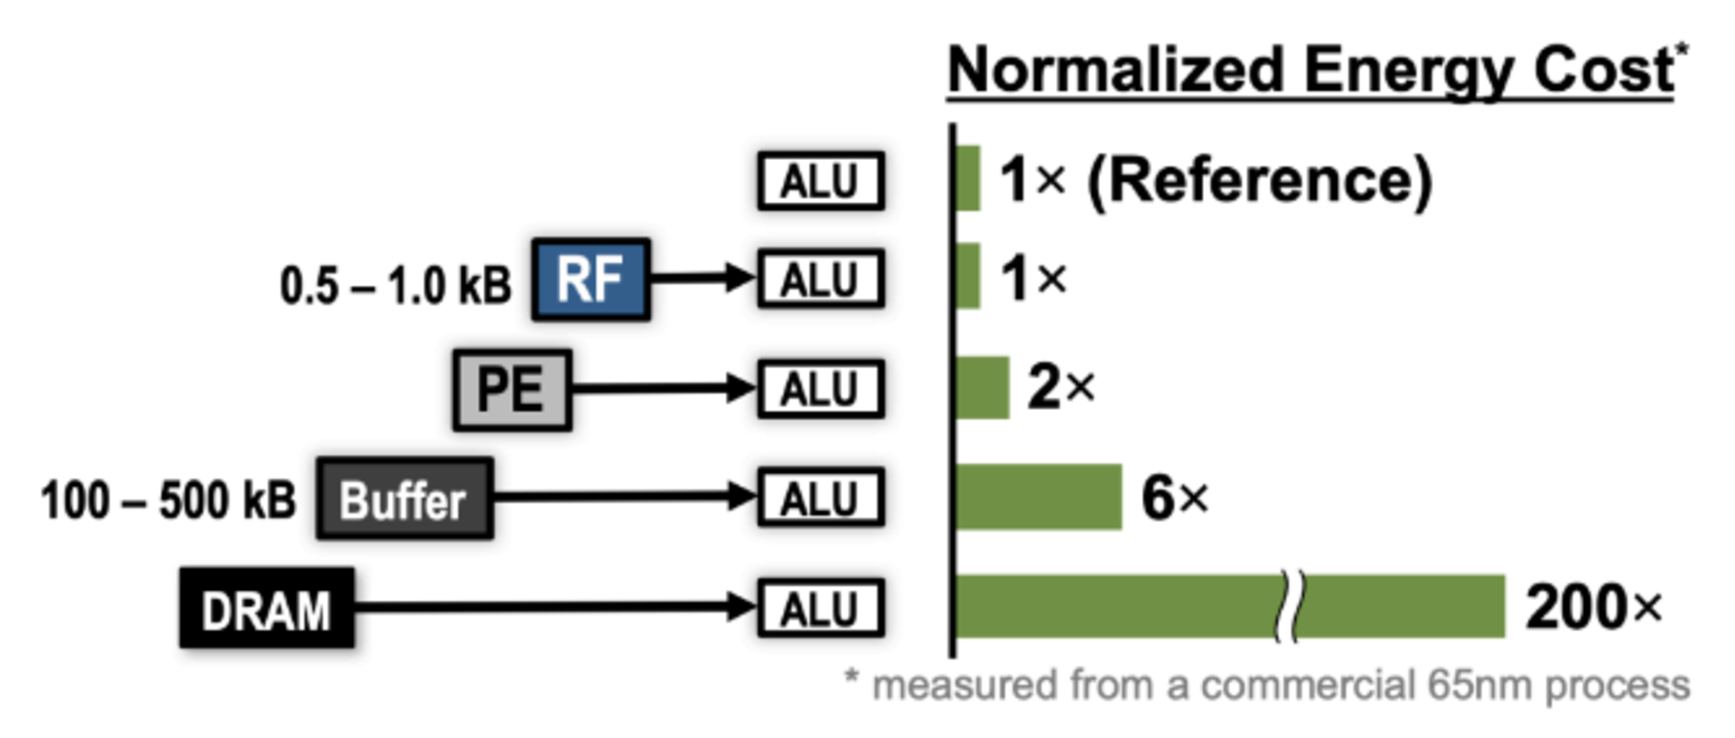
\includegraphics[width=\linewidth]{baseline_model.pdf}
  \end{center}
  \caption{Energy Baseline Model from Eyeriss\cite{eyerissv1}}
\end{figure}

\begin{figure}
  \begin{tabular}{ m{12em} | m{1cm}| m{5em} | m{1cm} }
    \textbf{Workload} & \textbf{Cycles} & \textbf{Total Energy (\textmu J)} & \textbf{Average Power (mW)} \\ \toprule
    16x16 Matmul & 1232 & 20 & 17.04 \\ \midrule
    64x64 Matmul & 18579 & 1016 & 54.6 \\ \midrule
    Smallest Layer (mobilenet) & 125573 & 16226 & 129.22 \\ \midrule
    Smallest Layer (resnet) & 922534 & 1114616 & 153.73 \\ \midrule
    Biggest Layer (mobilenet) & 7250444 & 149663 & 162.23 \\ \midrule
    \bottomrule
  \end{tabular}
  \caption{All layers are convolutional. Cycles are collected from RTL simulation.}
  \label{fig:spike_result}
\end{figure}

\subsection{Spike Power Model}
\subsubsection{Result}
We instrumented the DRAM, scratchpad, accumulator, MAC, and pipeline reg for their total access number throughout the workloads. We then run the workloads on RTL sim to collect the cycle counts and calculate the corresponding power described in Figure \ref{fig:spike_result} using the baseline model in Figure \ref{fig:baseline_model}.

\subsubsection{Spike Power Model vs Joules}
The power estimated from the spike power model only consists of the active dynamic power within Gemmini (\texttt{/Top/Tile/v}).
However, spike takes into account the SRAM read/write power whereas Joules leaves it out due to lack of internal power models in the fake asap7 SRAM .libs.
As a result, it is difficult to compare the power numbers across these 2 simulators.

However, in general, we can estimate that the runtime power of Gemmini is on the order of \textbf{10mW when idle} and goes up to \textbf{150mW when actively used}.
The power of Rocket is a tiny fraction of total system power (~3\%) and so it is fair to neglect it in the power model.
However, the L2 needs to be taken into account in the future since its energy isn't modeled in spike and Joules estimates that it contributes to nearly 20\% of the system power.

\subsection{Modeling Gemmini in Acceleregy}
\subsubsection{Gemmini Accelergy Model}
We modeled Gemmini's architecture as a combination of two scratchpads (weight and input), one accumulator scratchpad, and 16x16 PE elements; each with 8 bits integer MAC unit and register.

\begin{minted}[breaklines,fontsize=\small,frame=single]{yaml}
architecture:
  version: 0.3
  subtree:
    - name: eyeriss_like
      attributes:
        technology: 65nm
      local:
        - name: weights_sp
          class: SRAM
          attributes:
            width: 128
            depth: 4096
            n_banks: 2
            n_rdwr_ports: 1
        - name: ifmap_sp
          class: SRAM
          attributes:
            width: 128
            depth: 4096
            n_banks: 2
            n_rdwr_ports: 1
        - name: accum_sp
          class: SRAM
          attributes:
            width: 512
            n_banks: 1
            bank_depth: 1024
            depth: bank_depth * n_banks
            n_rdwr_ports: 1
      subtree:
      - name: PE[0..255]
        local:
          - name: weight_or_output
            class: reg
            attributes:
              datawidth: 8
          - name: mac
            class: intmac
            attributes:
              datawidth: 8
          - name: pipeline_reg
            class: reg
            attributes:
              datawidth: 8
\end{minted}


\section{Conclusion}

Made us realize that the Strober technique would actually be inefficient and inaccurate in this case. it works well for predicting average power on a very long timescale, but when Gemmini sees bursts of usage surrounded by times of exclusive CPU activity for pooling/im2col/dwconv/etc it will not be captured properly by a sampling methodology and peak power will not be observed. rather the best tool is a runtime power monitor that is pretrained on high and low toggle vectors on smaller benchmarks (like Simmani)

\subsection{Future Work}
The current Accelergy Gemmini model lacks of fidelity as it does not account for the behavior of the L2 cache, double buffering, wire, etc., so it will be a good idea to refine the existing model in the future.

\appendix
\section{Links}
% chipyard branch
We have a \texttt{power-modeling} branch on the main Chipyard repo (\texttt{github.com:ucb-bar/chipyard}) that contains the scripts to perform macroblock modeling of the MAC and evaluation of Rocket + Gemmini on Joules.
The Joules implementation is just copied/pasted TCL scripts for now, but we plan to make a proper Hammer plugin for it.

% esp-isa-sim fork
The spike power model is on a branch (\texttt{b\_progress}) of \texttt{esp-isa-sim} on a fork (\texttt{github.com:vighneshiyer/esp-isa-sim}).

% this repo

% models used for Accelergy

\section{Original Proposal}
The original proposal involved developing Strober\cite{strober}-like functionality for RTL designs by adding a few passes to the Golden Gate compiler to extract snippets of RTL trace data for long running simulations on an FPGA as seen in Figure \ref{fig:original_proposal}.
Those trace snapshots could be converted to gate-level activity and replayed on an energy simulator like Voltus to derive average power of a program during execution.
This required that a synthesis + pnr flow was up and running for asap7 for a large design such as Gemmini with Rocket.

\begin{figure}
  \centering
  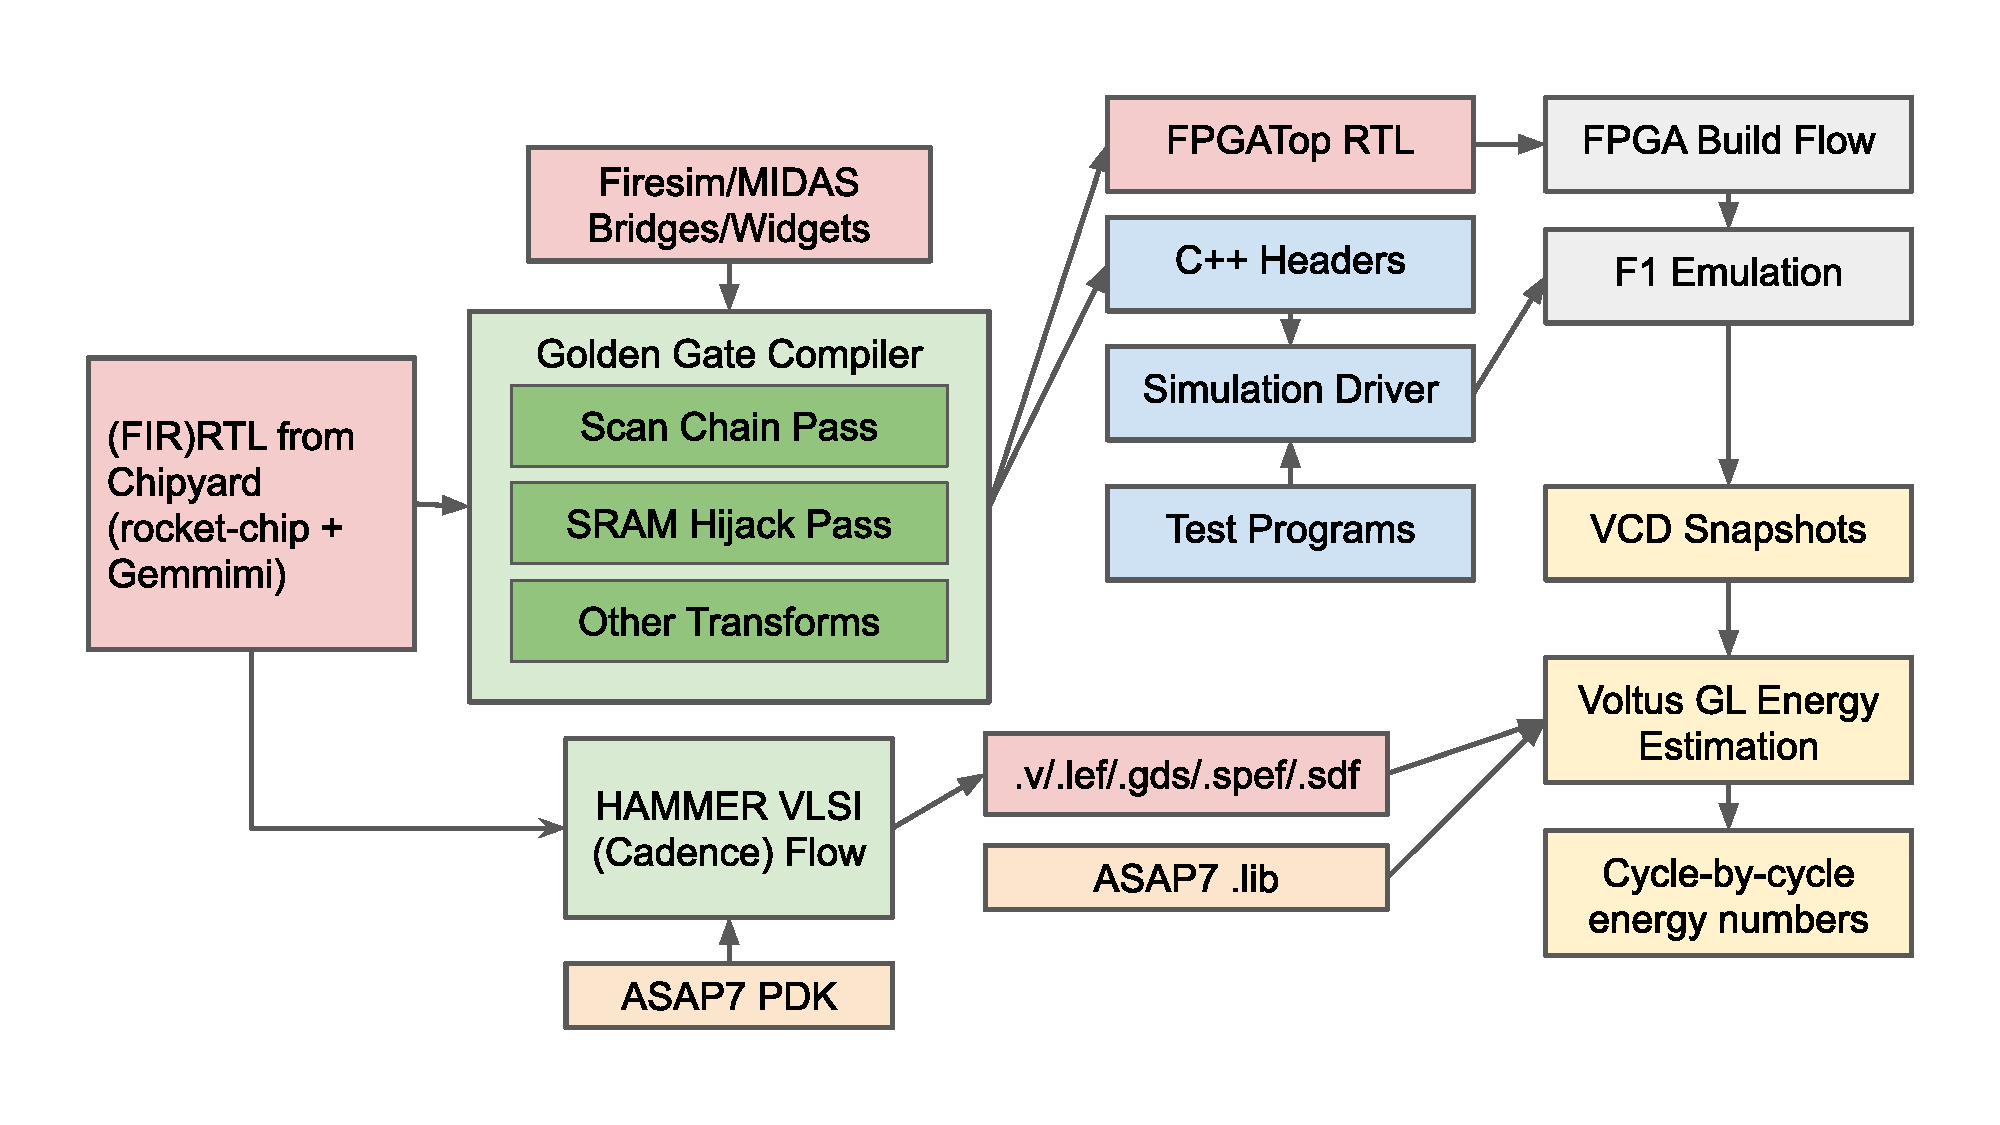
\includegraphics[width=\linewidth]{original_proposal.pdf}
  \label{fig:orignal_proposal}
  \caption{The original proposed flow}
\end{figure}

\subsection{Modifications / Rationale}
When we started the project, the focus was the `upper path' of the flow, which involves getting a set of Golden Gate passes, similar to the Strober DaisyChain pass, to work.
We ended up spending a lot of time in this area and were not able to make much progress due to our limited knowledge of the FIRRTL API and the complex nature of the codebase.
This work will have to wait until after the semester.

When we realized that the top flow was not viable by the end of the semester, we switched to trying to get the `bottom path' to work.
While working on that path, we figured that developing a simple activity-based power model embedded in spike was an easy way to validate the eventual results from the `bottom path'.
Later, as we struggled to get even Voltus working with Gemmini + Rocket and asap7, we switched to using Cadence Joules.

We planned to also use Accelergy to get a higher-fidelity power model than counting activities in spike.
In particular, Acceleregy could model the L2 as another memory cache layer, could model leakage power, and could model latency from DRAM to L2 to scratchpad and to the systolic mesh.
These latency numbers could be fetched from spike by instrumenting it with latency annotations from RTL sim or from RTL simulation directly.

\section{Prior Work}
STROBER\cite{strober} is a fast and cycle-accurate sample-based energy estimation framework that automatically transforms RTL into a deterministic FPGA simulator.
The work instruments the RTL design with a shadow scan chain that enables $\mu$Arch state extraction by the host.
To estimate energy, STROBER exploits the central limit theorem by taking state snapshots of the RTL at intervals using reservoir sampling and replaying those snapshots on a gate-level power simulator.

Simmani\cite{simmani} is a framework that trains a power model that takes toggle activity for a small subset of signals in the RTL design (found via clustering on signal toggle densities from training VCDs), instruments the RTL design with activity counters for these signals, and enables runtime power estimation.
This work demonstrated good power accuracy on running SqueezeNet on Rocket with a Hwacha vector accelerator.

DESSERT\cite{dessert} is a framework for FPGA-accelerated RTL debugging that enables synthesized assertions and full $\mu$Arch state dumping.
This work demonstrates the flexibility of a instrumented scan chain to dump arbitrary state that we could use to ``instrument" the RTL design in software after a bitstream has already been created.

%%
%% The acknowledgments section is defined using the "acks" environment
%% (and NOT an unnumbered section). This ensures the proper
%% identification of the section in the article metadata, and the
%% consistent spelling of the heading.
%\begin{acks}
%\end{acks}

%%
%% The next two lines define the bibliography style to be used, and
%% the bibliography file.
\bibliographystyle{ACM-Reference-Format}
\bibliography{references}

\end{document}
\endinput
%%
%% End of file `sample-sigconf.tex'.
